\chapter{Background}
Everyone knows what Wikipedia is and how to read an article, but there are many features
that most people are not aware of, \textit{e.g.} the possibility to see all the versions of a page. 
Anyone with a browser and can see and compare all the edits in a
Wikipedia page without much effort. For developers, there are many powerful resources, such as big datasets,
containing a lot more information.  

\section{History Exploration}
In the history section of a wikipedia article it's possibile to see every version of the page.
There are several tools anyone can use to explore the revision history: 
% questa va se vuoi foto e testo vicini
% \begin{wrapfigure}[12]{r}{0.5\textwidth}[h]
%     \centering
%     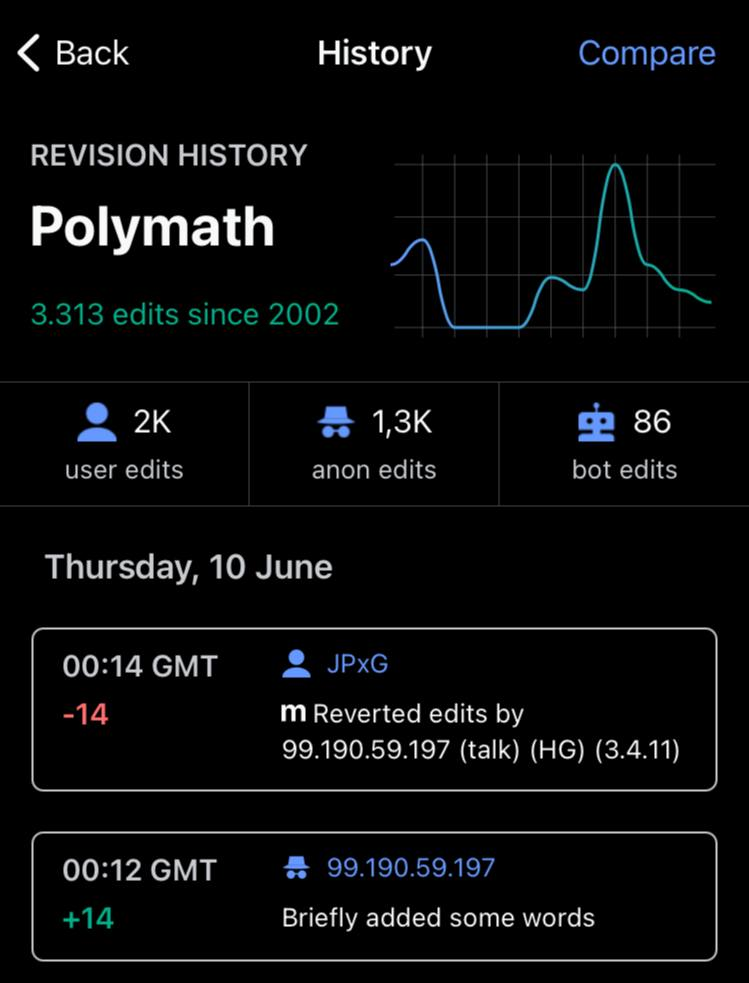
\includegraphics[width=0.35\textwidth]{./chapters/02/assets/mobile_history.jpg}
%     \caption{mobile interactive visualization of the history}
%     \label{fig:mobilehistory}
% \end{wrapfigure}


\begin{itemize}
    \item Mobile application: this resource is only available on mobile devices and provides us
        some statistics about the edits of the page, like the total number of revisions (Fig \ref{fig:mobilehistory}). 
    \item Website: it is possible to compare two versions with an interactive tool that shows us
        the progress of the modified page: each change corresponds to a bar indicating the number of
        bytes added or removed from the revision (Fig. \ref{fig:history}).
\end{itemize}

\begin{figure}[H]
    \centering
    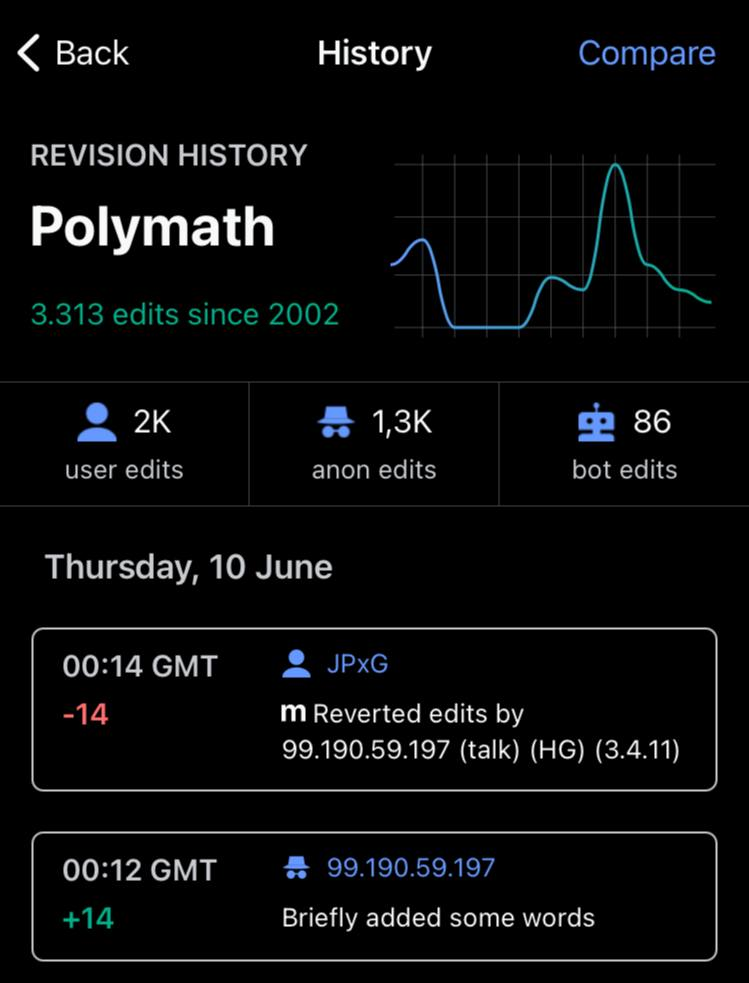
\includegraphics[width=0.35\textwidth]{./chapters/02/assets/mobile_history.jpg}
    \caption{Mobile interactive visualization of the history.}
    \label{fig:mobilehistory}
\end{figure}

\begin{figure}[H]
    \centering
    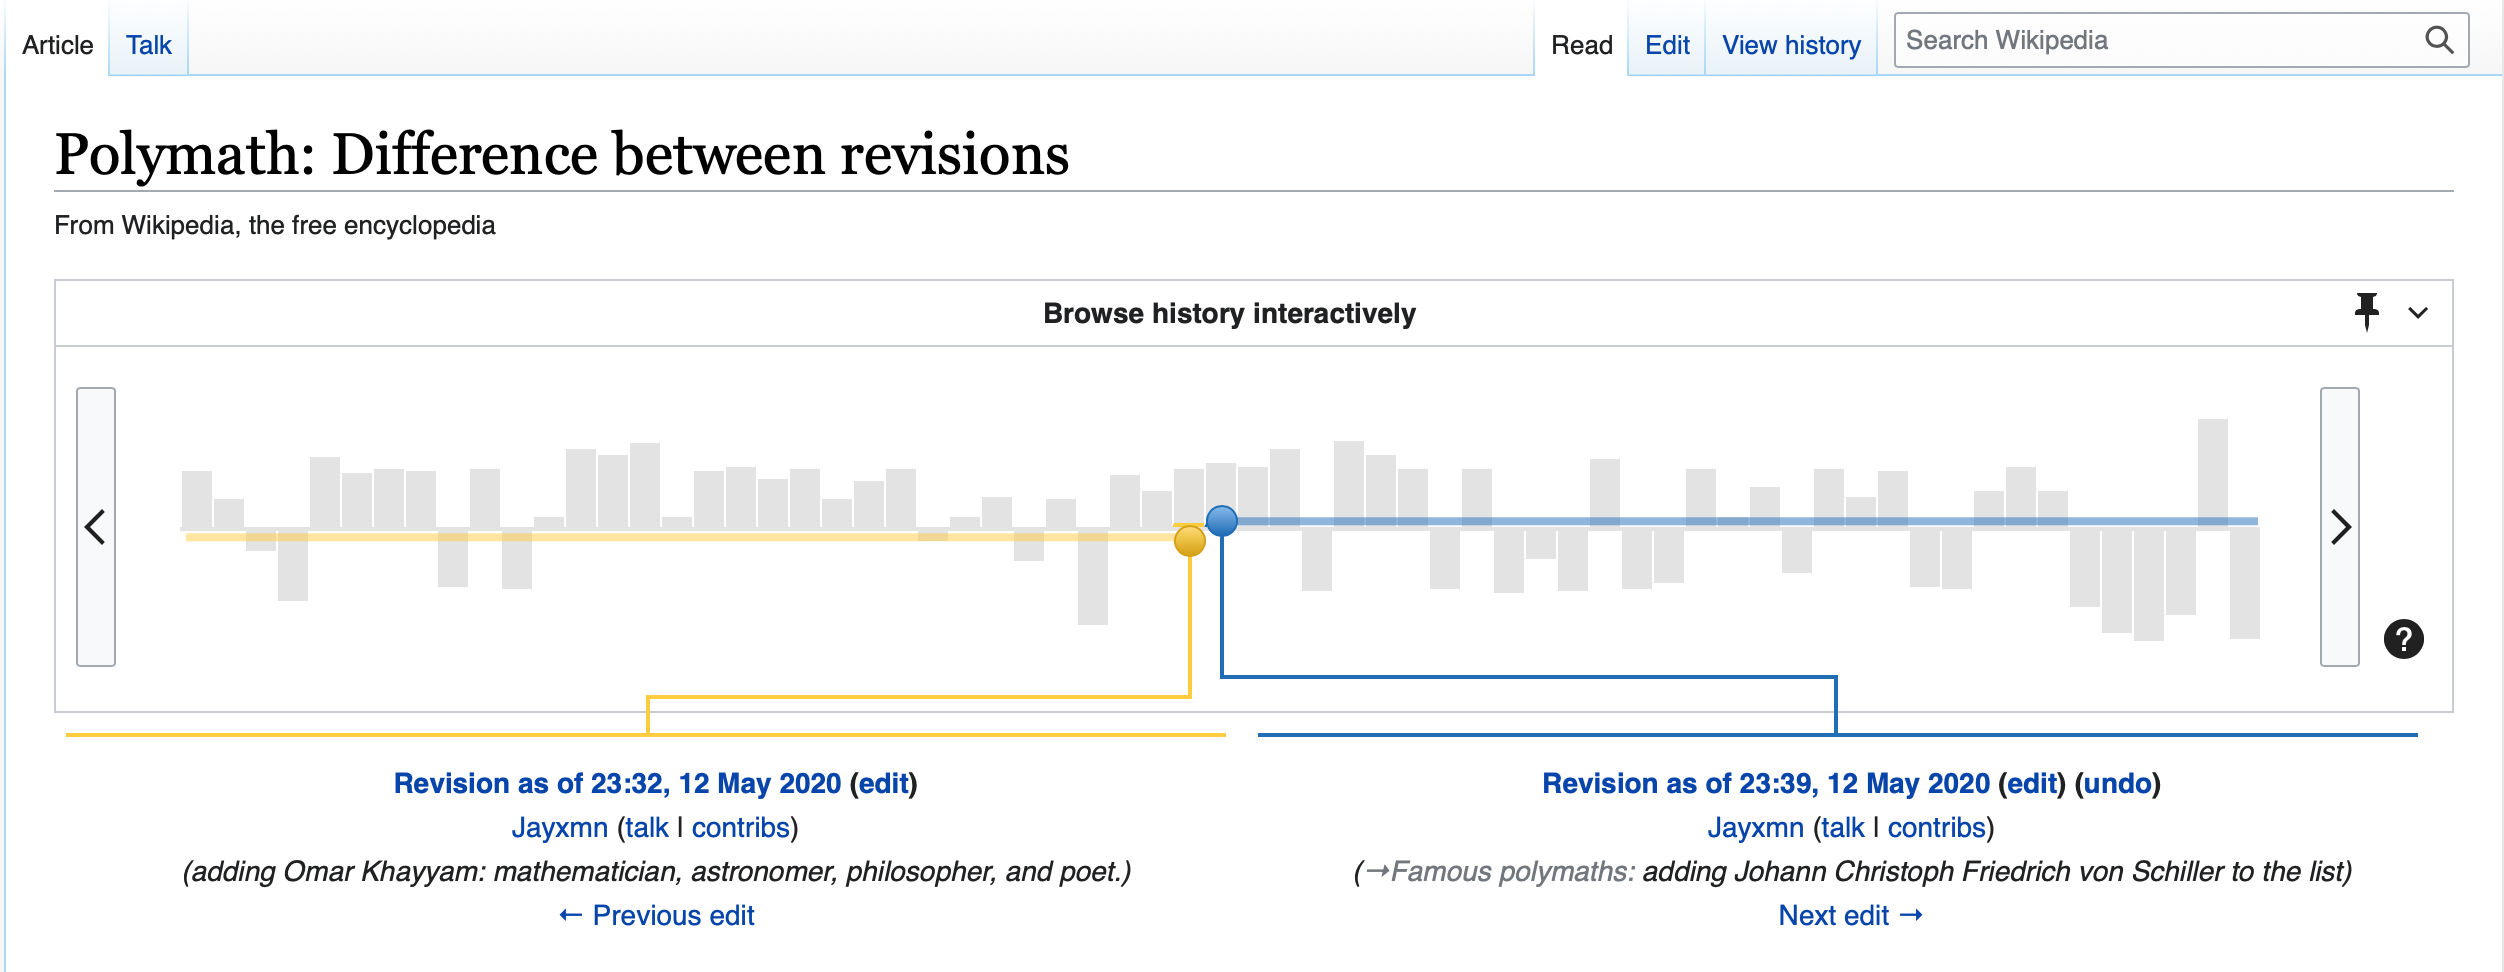
\includegraphics[width=1\textwidth]{./chapters/02/assets/history.png}
    \caption{Interactive visualization of the history.}
    \label{fig:history}
\end{figure}


\section{Dataset}
There are two datasets that store information about Wikipedia edits, that were made available by the WikiMedia
Foundation: a) the MediaWiki History\footnote{\url{https://wikitech.wikimedia.org/wiki/Analytics/Data_Lake/Edits/MediaWiki_history}} 
and b) the MediaWiki History Dumps \footnote{\url{https://wikitech.wikimedia.org/wiki/Analytics/Data_Lake/Edits/Mediawiki_history_dumps}}


The difference between the two (XML the former, TSV the latter) is that the first one also
contains the page content. The dataset used in this study is the MediaWiki History Dumps.\\

Each line of the TSV represent an event and, since it is denormalized, the events for user, page and
revision are stored in the same schema.
Event entities can be of different types:
\begin{itemize}
    \item Page: create, delete, move, restore or merge a page
    \item User: create, rename, altergroup (change user rights), alterblocks (block user)
    \item Revision: create (edit a page)
\end{itemize}

In this analysis we are only interested in revision events; they contain 68 fields but only a few of them are
needed. The entry could be divided in different sections: one section with general information about
the revision like timestamp and comment, a section with information about the user who did the
revision, one for the page where the revision was made, and the last one with more specific
information about the revision. The most relevant fields of each section are represented in the Tables 
\ref{table:user}, \ref{table:page}, \ref{table:revision}.The caption includes, if
needed, the descriptions of the fields.

\begin{table}[H]
    \centering
    \ra{1.2}
    \begin{tabularx}{\columnwidth}{@{}Xccccc@{}}
        \midrule
        \textbf{id} & \textbf{username} & \textbf{groups} & \textbf{is\_anonymous} & \textbf{registration} & \textbf{revision\_count}\\ \toprule
        42081 & Checco & autopatrolled & False & 2006-02-10 14:52:44.0 & 10420 \\

         \bottomrule
    \end{tabularx}
    
    \caption{Data about the user who made the revision. The \textit{groups} field helps to
     clearify if the user is an admin. The \textit{revision\_count} is needed to calculate complex metrics like M and G. \label{table:user}}
\end{table}


\begin{table}[H]
    \centering
    \ra{1.2}
    \begin{tabularx}{\columnwidth}{@{}Xccc@{}}
        \midrule
        \textbf{id} & \textbf{title} & \textbf{namespace} & \textbf{revision\_count} \\ \toprule
        116530 & Pino\_Rauti & 0 &  195 
        \\

         \bottomrule
    \end{tabularx}
    
    \caption{Data about the page where the revision took place. The \textit{namespace} field is used
    to filter only the revisions from the namespace 0, i.e., the actual encyclopedia. \label{table:page}}
\end{table}

\begin{table}[H]
    \centering
    \ra{1.2}
    \begin{tabularx}{\columnwidth}{@{}Xcccc@{}}
        \midrule
        \textbf{id} & \textbf{parent\_id} & \textbf{is\_reverted} & \textbf{reverter\_id} & \textbf{is\_reverter} \\ \toprule
        73507165 & 73506955 & True &  73511400 & False 
        \\

         \bottomrule
    \end{tabularx}
    
    \caption{Data about the revision itself, we are able to identify if the revision is reverting another
    one, if it is been reverted and who is the reverter. \label{table:revision} }
\end{table}


\begin{table}[H]
    \centering
    \ra{1.2}
    \begin{tabularx}{\columnwidth}{@{}Xc@{}}
        \midrule
        \textbf{language} & \textbf{size}\\ \toprule
        English & 540 GB \\
        Spanish & 72 GB \\
        Italian & 54 GB \\
        Catalan & 12 GB \\

         \bottomrule
    \end{tabularx}
    
    \caption{Size of the dataset in different languages. \label{table:datasetsize}}
\end{table}

\section{Definitions}
It is worth defining some terms that will be used several times in the discussion.
\newtheorem{Definition}{Definition}
\begin{Definition}
    (Revert) On Wikipedia, reverting means undoing or otherwise negating the effects of one or more edits,
    which results in the page (or a part of it) being restored to a previous version.\footnote{\url{https://en.wikipedia.org/wiki/Help:Reverting}} % TODO: citare il sito 
\end{Definition}

\begin{Definition}
    (Revert chain) On a Wikipedia page, a revert chain occurs when an edit that reverts an edit is itself reverted.
\end{Definition}

\begin{Definition}
    (Mutual revert) A “mutual revert” is recognized if a pair of editors (x, y) is observed once with x and once with y as the reverter~\cite{Yasseri2014}.
\end{Definition}

\begin{Definition}
    (Editor weight) The weight of an editor x is defined as the number of edits N performed by him or her~\cite{Yasseri2014}.
\end{Definition}

\begin{Definition}
    (Mutual revert weight) The weight of a mutually reverting pair MW is defined as the minimum of the weights of the two editors~\cite{Yasseri2014}.
\end{Definition}

\begin{Definition}
    (Chain weight) The weight of a revert chain CW is defined as the minimum of the weights of the editors involved in the chain.
\end{Definition}


\section{Metrics}
Two complex controversiality metrics have been computed in this study: the first one, M, is a state of the
art metric introduced by Yasseri \textit{et al.}~\cite{Yasseri2014} which gives us a score of the controversiality of the page
based on the presence of mutual reverts. On the other hand the one that we designed, called G, is very similar to M, but
instead of using mutual reverts, it uses reverts chains to evaluate the controversiality of the page.  

\paragraph*{Controversiality M}
The controversiality M of an article is defined by summing the weights of all the mutually reverting
editors pairs, excluding the topmost pair, and multiplying this number by the total number of
editors E involved in the article. Using the number of edits as user weight allows us to focus on
experienced users, the higher is the edit count the higher the value of the M metric will be. This
is also useful to exclude the anonymous users since their edit count is equal to zero.

\begin{equation}
    M = E   \sum_{all\ mutual\ reverts} MW
\end{equation}

\paragraph*{Controversiality G}
The controversiality G of an article is defined by summing the weights of all the chains
there are on a page and by multiplying this number by the total number of editors N involved in at least one chain.
Similarly to M, thanks to users' edit count, the weight of chains with anonymous users involved will be 0.
\begin{equation}
    G = N \sum_{all\ revert\ chains} CW
\end{equation}




